% ===========================================
% Template for ICMC 2021 in Santiago, Chile (version1)
% adapted from earlier LaTeX paper templates for the ICMC, SMC, etc...
% by Rodrigo F. Cádiz rcadiz@uc.cl
% ===========================================

\documentclass{article}
\usepackage{icmc2021template}
\usepackage{times}
\usepackage{ifpdf}
\usepackage{soul}
\usepackage[english]{babel}
\usepackage{enumitem}
\usepackage{musicography}
\usepackage{amsmath}
\usepackage{arydshln}
\usepackage{caption}
\captionsetup{skip=5pt}
%\usepackage{cite}

%%%%%%%%%%%%%%%%%%%%%%%% Some useful packages %%%%%%%%%%%%%%%%%%%%%%%%%%%%%%%
%%%%%%%%%%%%%%%%%%%%%%%% See related documentation %%%%%%%%%%%%%%%%%%%%%%%%%%
%\usepackage{amsmath} % popular packages from Am. Math. Soc. Please use the 
%\usepackage{amssymb} % related math environments (split, subequation, cases,
%\usepackage{amsfonts}% multline, etc.)
%\usepackage{bm}      % Bold Math package, defines the command \bf{}
%\usepackage{paralist}% extended list environments
%%subfig.sty is the modern replacement for subfigure.sty. However, subfig.sty 
%%requires and automatically loads caption.sty which overrides class handling 
%%of captions. To prevent this problem, preload caption.sty with caption=false 
%\usepackage[caption=false]{caption}
%\usepackage[font=footnotesize]{subfig}

% ====================================================
% ================ Define title and author names here ===============
% ====================================================
%user defined variables
\def\papertitle{MusAssist: A Domain Specific Language for Music Notation}
\def\firstauthor{Ilana Shapiro}
\def\secondauthor{Second Author}
\def\thirdauthor{Third Author}
\def\fourthauthor{Fourth Author}
\def\fifthauthor{Fifth Author}
\def\sixthauthor{Sixth Author}

% adds the automatic
% Saves a lot of output space in PDF... after conversion with the distiller
% Delete if you cannot get PS fonts working on your system.

% pdf-tex settings: detect automatically if run by latex or pdflatex
\newif\ifpdf
\ifx\pdfoutput\relax
\else
   \ifcase\pdfoutput
      \pdffalse
   \else
      \pdftrue
  \fi
\fi

\ifpdf % compiling with pdflatex
  \usepackage[pdftex,
    pdftitle={\papertitle},
    pdfauthor={\firstauthor, \secondauthor, \thirdauthor},
    bookmarksnumbered, % use section numbers with bookmarks
    pdfstartview=XYZ % start with zoom=100% instead of full screen; 
                     % especially useful if working with a big screen :-)
   ]{hyperref}
  %\pdfcompresslevel=9

  \usepackage[pdftex]{graphicx}
  % declare the path(s) where your graphic files are and their extensions so 
  %you won't have to specify these with every instance of \includegraphics
  \graphicspath{{./figures/}}
  \DeclareGraphicsExtensions{.pdf,.jpeg,.png}

  \usepackage[figure,table]{hypcap}

\else % compiling with latex
  \usepackage[dvips,
    bookmarksnumbered, % use section numbers with bookmarks
    pdfstartview=XYZ % start with zoom=100% instead of full screen
  ]{hyperref}  % hyperrefs are active in the pdf file after conversion

  \usepackage[dvips]{epsfig,graphicx}
  % declare the path(s) where your graphic files are and their extensions so 
  %you won't have to specify these with every instance of \includegraphics
  \graphicspath{{./figures/}}
  \DeclareGraphicsExtensions{.eps}

  \usepackage[figure,table]{hypcap}
\fi

%setup the hyperref package - make the links black without a surrounding frame
\hypersetup{
    colorlinks,%
    citecolor=black,%
    filecolor=black,%
    linkcolor=black,%
    urlcolor=black
}


% ====================================================
% ================ Title and author info starts here ===============
% ====================================================
% Title.
% ------
\title{\papertitle}

% Authors
% Please note that submissions are anonymous, therefore 
% authors' names should not be VISIBLE in your paper submission.
% They should only be included in the camera-ready version of accepted papers.
% uncomment and use the appropriate section (1, 2 or 3 authors)
%
% Single address
% To use with only one author or several with the same address
% ---------------
%\oneauthor
%   {\firstauthor} {Affiliation \\ %
%     {\tt \href{mailto:author@uc.cl}{author@uc.cl}}}

%Two addresses
% the default spacing is 1.5in, but this can be reduced to 0.5in or less, if needed
%--------------
% \twoauthors
%   {1.5in}
%   {\firstauthor} {Affiliation1 \\  %
%     {\tt \href{mailto:author1@uc.cl}{author1@uc.cl}}}
%   {\secondauthor} {Affiliation2 \\  %
%     {\tt \href{mailto:author2@uc.cl}{author2@uc.cl}}}

% Three addresses
% the default spacing is 0.5in, but this can be reduced to 0.3in or less, if needed
% --------------
 \oneauthor
  %  {0.5in}
   {\firstauthor} {Pomona College \\ %
     {\tt \href{mailto:issa2018@mymail.pomona.edu}{issa2018@mymail.pomona.edu}}}
  %  {\secondauthor} {Affiliation2 \\ %
  %    {\tt \href{mailto:author2@myorg.org}{author2@myorg.org}}}
  %  {\thirdauthor} { Affiliation3 \\ %
  %    {\tt \href{mailto:author3@myorg.org}{author3@myorg.org}}}

% Four addresses
% the default spacing is 1.5in, but this can be reduced to 0.5in or less, if needed
% --------------
% \fourauthors
%   {1.5in}
%   {\firstauthor} {Affiliation1 \\ %
%     {\tt \href{mailto:author1@uc.cl}{author1@uc.cl}}}
%   {\secondauthor} {Affiliation2 \\ %
%     {\tt \href{mailto:author2@uc.cl}{author2@uc.cl}}}
%   {\thirdauthor} { Affiliation3 \\ %
%     {\tt \href{mailto:author3@uc.cl}{author3@uc.cl}}}
%   {\fourthauthor} { Affiliation4 \\ %
%     {\tt \href{mailto:author4@uc.cl}{author4@uc.cl}}}

% Five addresses
% the default spacing is 0.5in, but this can be reduced to 0.3in or less, if needed
% --------------
% \fiveauthors
%   {0.5in}
%   {\firstauthor} {Affiliation1 \\ %
%     {\tt \href{mailto:author1@uc.cl}{author1@uc.cl}}}
%   {\secondauthor} {Affiliation2 \\ %
%     {\tt \href{mailto:author2@uc.cl}{author2@uc.cl}}}
%   {\thirdauthor} { Affiliation3 \\ %
%     {\tt \href{mailto:author3@uc.cl}{author3@uc.cl}}}
%   {\fourthauthor} { Affiliation4 \\ %
%     {\tt \href{mailto:author4@uc.cl}{author4@uc.cl}}}
%   {\fifthauthor} { Affiliation5 \\ %
%     {\tt \href{mailto:author5@uc.cl}{author5@uc.cl}}}

% Six addresses
% the default spacing is 0.5in, but this can be reduced to 0.3in or less, if needed
% --------------
% \sixauthors
%   {0.5in}
%   {\firstauthor} {Affiliation1 \\ %
%     {\tt \href{mailto:author1@uc.cl}{author1@uc.cl}}}
%   {\secondauthor} {Affiliation2 \\ %
%     {\tt \href{mailto:author2@uc.cl}{author2@uc.cl}}}
%   {\thirdauthor} { Affiliation3 \\ %
%     {\tt \href{mailto:author3@uc.cl}{author3@uc.cl}}}
%   {\fourthauthor} { Affiliation4 \\ %
%     {\tt \href{mailto:author4@uc.cl}{author4@uc.cl}}}
%   {\fifthauthor} { Affiliation5 \\ %
%     {\tt \href{mailto:author5@uc.cl}{author5@uc.cl}}}
%   {\sixthauthor} { Affiliation6 \\ %
%     {\tt \href{mailto:author6@uc.cl}{author6@uc.cl}}}


% ====================================================
% =============== The document content starts here ===============
% ====================================================
\begin{document}
%
\capstartfalse
\maketitle
\capstarttrue
%
\begin{abstract}
MusAssist is an external, declarative domain specific language for music notation. 
Users can change key signatures, start a new measure, and describe musical structures 
such as notes, rests, and custom chords in MusAssist’s straightforward syntax much in 
the same way they would when composing. MusAssist is unique in that users can also describe 
complex musical templates for triads and seventh chords, cadences, and the four primary 
harmonic sequences with desired length. The level of abstraction of a MusAssist template 
MusAssist matches that of the theoretical musical structure it describes (e.g. users can describe
 a harmonic sequence without lowering the abstraction level to chords and notes). This allows 
 users to write out specifications precisely at the conceptual levels of the musical structures 
 they would organically conceive when composing by hand. The musical expressions described by 
 the specifications are expanded out (i.e. the level of abstraction is fully lowered) by the 
 Haskell-based MusAssist compiler and are translated to MusicXML, a language accepted by most 
 major notation software, allowing for further manual editing. 
\end{abstract}
%

\section{Introduction}\label{sec:introduction}
When writing music, composers must manually transition from musical theoretical concepts to notes on a page.
This process can be tedious and slow, requiring the composer to expand complex structures, such as cadences and sequences,
by hand to the notes that they constitute. The level of abstraction of the musical theoretical structure is 
higher than what the composer actually writes. 

Domain specific languages, or DSLs, 
are programming languages highly specialized for a specific application and thus characterized by limited expressiveness.
An $external$ $DSL$ has custom syntax that is separated from the primary language of its application. 
MusAssist is an external, declarative domain specific language (DSL) for music notation that attempts bridge the divide between
music theory and notation. Users describe a composition in MusAssist's straightforward syntax, and 
the MusAssist compiler writes out the music via these instructions. MusAssist's declarative programming 
paradigm was chosen to correspond with the declarative nature of handwritten music. 

Fundamentally, MusAssist supports notes (including rests) and custom chords (i.e. any desired collection of notes)
in the octave and key of choice, as well as change the key signature or start a new measure at any
point. MusAssist is unique in that users can also write specifications for complex musical templates \textit{at the same level of abstraction
as the musical theoretical structures they describe}. MusAssist supports \textbf{chords} (all triads and seventh chords in any inversion), \textbf{cadences}
(perfect authentic, imperfect authentic, plagal, half, deceptive), and \textbf{harmonic sequences} (ascending
fifths, descending fifths, ascending 5-6, descending 5-6) of a desired length. The musical expression 
described by this specification is completely expanded out (i.e. the level of abstraction is
fully lowered) by the Haskell-based MusAssist compiler.

The target language of the MusAssist compiler is MusicXML, itself a DSL that is an extension of
XML (Extensible Markup Language). MusicXML is accepted by most major notation software programs (such as MuseScore). 
Thus users can open can open the resulting MusicXML file of a compiled MusAssist composition in MuseScore or another
program for further customization and editing, thus bypassing the need to write out complex musical templates by hand at a 
note- and chord-level of abstraction. Beyond a professional music compositional aid, MusAssist may be particularly 
helpful to music theory students as an educational tool, enabling them to visualize the relationship between a theortical musical structure 
and its expanded form, such as a cadence and the chords resulting from its expansion.


\section{Related Work}\label{sec:related_work}

The era of music DSLs began in 2008 with Ge Wang's ChucK audio processing language, which  
spans the application domains of ``methods for sound synthesis, physical modeling of real-time world artifacts and spaces (e.g., 
musical instruments, environmental sounds), analysis and information retrieval of sound and music, to 
mapping and crafting of new controllers and interfaces (both software and physical) for music, 
algorithmic/generative processes for automated or semi-automatic composition and accompaniment, [and] 
real-time music performance." %\citeparen{wang_2008}. 
Since then, researchers have taken advantage of the increased flexibility afforded to DSLs via their limited expressiveness to create
music DSLs tailored towards notation, algorithmic composition, signal processing, live coding with music performance, and more. In the 
 notation domain, MusicXML, LilyPond, and PyTabs stand out.

Michael Good's MusicXML is an Internet-friendly, XML-based, declarative DSL capable of representing Western music 
notation and sheet music since c. 1600. 
It acts as an "interchange format for applications in music notation, music analysis, music information retrieval, 
and musical performance," thus supporting sharing between specialized applications. %\cite{good_2013}

MusicXML attempts to emulate for online sheet music and music software what the popular MIDI format 
did for electronic instruments. It is derived from XML in order to help solve the music 
interchange problem: to create a standardized method to represent complex, structured data in order to support 
smooth interchange between "musical notation, performance, analysis, and retrieval applications." XML has the 
desired qualities of "straightforward usability over the Internet, ease of creating documents, and human readability" 
that translate directly into the musical domain, and it is more powerful and expressive 
than MIDI. %\cite{good_2001}

MusicXML is more expressive than MusAssist, but the
level of abstraction of all musical elements is extremely low (i.e. chords must be written out 
as individual notes) and its syntax is very difficult and tedious to write by hand. However,
its flexibility and expressiveness make MusicXML an excellent target 
compilation language for MusAssist's user-friendly syntax and high-level musical theoretical templates.

LilyPond, an external declarative DSL created by Han-Wen Nienhuys and 
Jan Nieuwenhuizen, is similar to MusAssist. It features a "modular, extensible and programmable 
compiler" written in Scheme to generate Western music notation of excellent quality and supports the mixing of text and music elements. 
Text-based \textit{musical expressions}, or fragments of music with 
set durations, are compiled to an aesthetically formatted score.

LilyPond and MusAssist are both music notation DSLs tailored to non-programming audiences. However, 
they differ in two fundamental areas: 
(1) MusAssist supports complex music templates at the levels of abstraction of the 
musical structures they represent, whereas LilyPond only supports 
more granular, low level composition of individual notes and chords, and (2) the output of the MusAssist compiler is intentionally editable via
notation software, unlike LilyPond's compiler, which produces a static, printable PostScript or PDF file by 
taking in a file with a formal representation of the desired music.
%\cite{nienhuys_nieuwenhuizen_2003}.

Simic et al.'s external, declarative DSL PyTabs similarly is geared toward music notation, but in a different
domain than MusAssist. Specifically, 
the authors attempt to solve visual problem of  tablature  notation, 
and the lack of standardization of how  to specify note duration in this format, by consolidating 
these issues into a formal language. Tablature notation is outside the scope of MusAssist's focus on Western 
musical theoretical structures.
 % \citeparen{simic_bal_dejanovic_vaderna}.

\section{Language Features}\label{sec:language_features}
\subsection{Low-Level Fundamentals}
On the most basic level, MusAssist supports individual notes and rests. Rests are  
given a duration from sixteenth to whole note, and notes are further defined by note name (A to G), 
accidental (from double flat to double flat), and octave (1 to 8, after the range of a piano).
Just as in normal notation, the absence of an accidental indicates natural quality.
Finally, users can also define ``custom chords,'' or user-defined collections of individual notes.
These are not considered templates as the high-level description of the chord is not given.

\subsection{High-Level Templates}
MusAssist's supports templates for chords, cadences, harmonic sequences, specified uniquely
at the abstraction level of the musical theoretical structures they represent. 

Precisely as in music theory, chords are specified by root note (defined as the fundamental note is),
quality (major, minor, augmented, diminished, or half diminished), 
inversion (root, first, second, or third), and chord type (triad or seventh). 
Half diminished and third inversion options apply to seventh chords only. The root note 
cannot have a double accidental, as this can introduce triple accidentals in the chord, which MusAssist
does not support.

Cadences are specified by cadence type (perfect or imperfect authentic, half, plagal, 
or deceptive) and key (defined by a fundamental note and a quality, either major or minor). 
Currently, MusAssist only supports a single treble clef line. Thus, cadences are written out in the 
upper voices only, in keyboard voice leading style and incorporating principles of smooth voice leading.

Based on the principles of functional harmony, there are several ways to represent a cadence. 
In MusAssist, the following representations were chosen. The major version is presented first, 
and the minor after that, in parentheses.

\begin{table}[h]
  \begin{center}
    \renewcommand{\arraystretch}{1.5}
\begin{tabular}{|l|l|}
\hline
Perfect Authentic & IV-V-I (iv-V-i) \\ \hline
Imperfect Authentic & IV-vii$^{\text{o}{6 \atop 4}}$-I$^{6 \atop 4}$ (iv-vii$^{\text{o}{6 \atop 4}}$-i$^{6 \atop 4}$) \\ \hline
Plagal & IV$^{6 \atop 4}$-I (iv$^{6 \atop 4}$-I) \\ \hline
Deceptive & IV-V$^{6 \atop 4}$-vi$^{6 \atop 4}$ (iv-V$^{6 \atop 4}$-VI$^{6 \atop 4}$) \\ \hline
Half & IV-ii$^6$-V (iv-ii$^{\text{o}6}$-V) \\ \hline
\end{tabular}
\caption{MusAssist Cadences Summary}
\end{center}
\label{table:cadences}
\vspace{-7mm}
\end{table}

All cadences except perfect authentic are built exclusively with triads.
Perfect authentic cadences also double the root in the final chord to simulate the 4-5-1 bass line
as well as to preserve the requisite 2-1 downward step in the uppermost voice. 
This is demonstrated in \figref{fig:perfauth}, produced with the MusAssist syntax \\
\noindent\verb.(PerfAuthCadence Eb5 min sixteenth). \\
when compiled and loaded into MuseScore notation software.
\begin{figure}[h!]
\centering
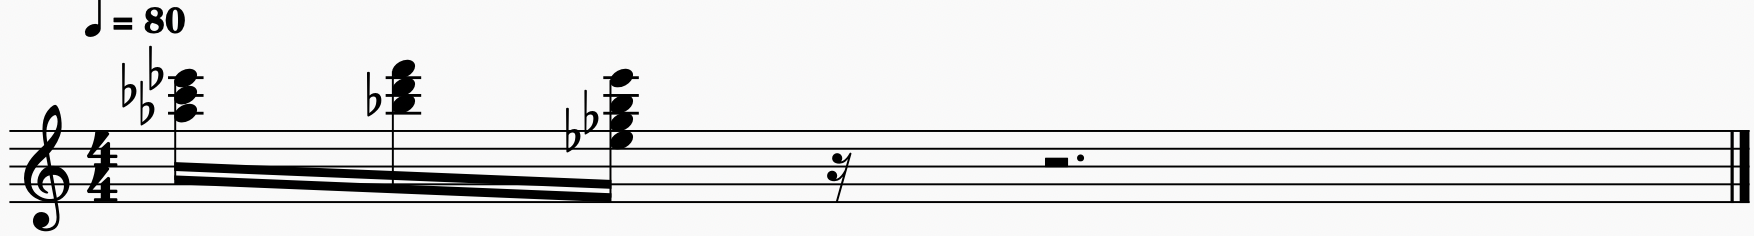
\includegraphics[width=0.45\textwidth]{images/perfauth}
  \caption{Perfect Authentic Cadence in E\musFlat\; minor \label{fig:perfauth}}
\end{figure}

Finally, harmonic sequences are specified by harmonic sequence type (ascending fifths,
descending fifths, ascending 5-6, descending 5-6), key (just as in cadences), duration of each chord,
and length of the sequence. Since MusAssist does not yet support multi-line composition, harmonic sequences are 
writte like cadences in keyboard-style voice leading. Though the
upper-voice harmonization of a harmonic sequence need not follow the direction in the sequence’s
name, MusAssist chooses a chord inversion and voice leading pattern such that each sequence does
align with the direction of its name (i.e. ascending sequences will ascend directionally) 
and also maximizes smooth voice leading.

In music theory, harmonic sequences can be implemented in several ways depending on desired inversion scheme. 
The chosen chord progressions for each MusAssist sequence are summarized in \tabref{table:harmseq}.
All sequences are shown in major for the sake of example, but their inverse in minor is equally supported. 
Each consists of fourteen distinct chords before repeating in the subsequent octave. 

\begin{table}[h!]
  \begin{center}
  \begin{tabular}{|c|@{}c@{}|}
  \hline
  Ascending Fifths  & \renewcommand{\arraystretch}{1.5}
                    \begin{tabular}{lllll} 
                        I$^{6 \atop 4}$ & V                & ii$^{6 \atop 4}$            & vi              & iii$^{6 \atop 4}$ \\ \hdashline
                        vii$^\text{o}$  & IV$^{6 \atop 4}$ & I                           & V$^{6 \atop 4}$ & ii                \\ \hdashline
                        vi$^{6 \atop 4}$ & iii             & vii$^{\text{o}{6 \atop 4}}$ & IV              
                    \end{tabular} \\ \hline 
  Descending Fifths & \renewcommand{\arraystretch}{1.5}
                    \begin{tabular}{lllll} 
                      I                & IV$^{6 \atop 4}$ & vii$^\text{o}$  & iii$^{6 \atop 4}$ & vi                          \\ \hdashline
                      ii$^{6 \atop 4}$ & V                & I$^{6 \atop 4}$ & IV                & vii$^{\text{o}{6 \atop 4}}$ \\ \hdashline
                      iii              & vi$^{6 \atop 4}$ & ii              & V$^{6 \atop 4}$
                    \end{tabular} \\ \hline
  Ascending 5-6     & \renewcommand{\arraystretch}{1.5}
                    \begin{tabular}{lllll} 
                      I     & vi$^6$ & ii              & vii$^{\text{o}6}$ & iii      \\ \hdashline
                      I$^6$ & IV     & ii$^6$          & V                 & iii$^6$  \\ \hdashline 
                      vi    & IV$^6$ & vii$^\text{o}$  & V$^6$           
                    \end{tabular} \\ \hline
  Descending 5-6    & \renewcommand{\arraystretch}{1.5}
                    \begin{tabular}{lllll} 
                      I$^{6 \atop 4}$ & V                & vi$^{6 \atop 4}$ & iii                         & IV$^{6 \atop 4}$ \\ \hdashline 
                      I               & ii$^{6 \atop 4}$ & vi               & vii$^{\text{o}{6 \atop 4}}$ & IV               \\ \hdashline 
                      V$^{6 \atop 4}$  & ii               & iii$^{6 \atop 4}$           & vii$^\text{o}$  
                    \end{tabular} \\ \hline
  \end{tabular}
  
  \caption{MusAssist Harmonic Sequences Summary\label{table:harmseq}}
  
\end{center}

\end{table}

\vspace{-8mm}
\subsection{Additional Features}
Beyond compositional elements, users can set the key signature at the beginning
of any measure up to seven sharps or flats by specificing note name, accidental, and quality (sharp or flat).
Users can also start a new measure or create a blank measure. Finally,
users can label MusAssist expressions and reuse them later in the program. MusAssist
comments are designated with \verb!\\!.

All compiled MusAssist programs adhere to standard notation style. Tied notes and rests 
are broken up greedily into valid durations ordered either greatest to least (for tied
notes/rests spilling into the beginnings of measures), or least to greatest in all
other cases. The tempo for all MusAssist programs
is set at \musQuarter\;= 80bpm and cannot currently be customized or changed.

\section{Sample Programs}
The following examples present MusAssist syntax followed by the result of
 opening the compiled MusicXML code in MuseScore. 
They demonstrate (1) the complexity that MusAssist is capable of and (2) 
that MusAssist programs can certainly sound diatonic and pleasing to the ear.

\section{Example 1}
\begin{figure}[h!]
\begin{verbatim}
SET_KEY Amaj
(D4 whole) (F#4 quarter) (Ab4 quarter) 
      (G#4 eighth) (rest sixteenth)           
// this is a comment
notes1 = (D4 whole) (F#4 quarter) 
      (Ab4 quarter) (G#4 eighth) (rest whole)  
// note without b or # is considered 
  to be natural chords1 = ([Bbb5, Db5, C5] half) ([C#5, E5] half) 
      (C6 min triad inv:first quarter) 
(F#4 halfdim seventh inv:second eighth)
(D4 whole) (F#4 quarter) (Ab4 quarter) (G##4 eighth) (rest sixteenth)
([Bbb5, Db5, C5] half) ([C#5, E5] half) (C6 min triad inv:first quarter) 
(F#4 halfdim seventh inv:second eighth)
SET_KEY Dmin
NEW_MEASURE
(DescFifths G5 min quarter length:15) (PerfAuthCadence Eb5 min half)
notes1 chords1 (AscFifths G3 min quarter length:5) chords1 
(PerfAuthCadence Eb5 min sixteenth) chords1
\end{verbatim}
\caption{MusAssist Syntax}
\end{figure}
kjsfdh sdkhf dskhf lsakj hdfakjs,d fhkwaj,es hdfuakwj,smdh luawksj,mdh 
kjsfdh sdkhf dskhf lsakj hdfakjs,d fhkwaj,es hdfuakwj,smdh luawksj,mdh 
kjsfdh sdkhf dskhf lsakj hdfakjs,d fhkwaj,es hdfuakwj,smdh luawksj,mdh 
kjsfdh sdkhf dskhf lsakj hdfakjs,d fhkwaj,es hdfuakwj,smdh luawksj,mdh 
kjsfdh sdkhf dskhf lsakj hdfakjs,d fhkwaj,es hdfuakwj,smdh luawksj,mdh 
kjsfdh sdkhf dskhf lsakj hdfakjs,d fhkwaj,es hdfuakwj,smdh luawksj,mdh 
kjsfdh sdkhf dskhf lsakj hdfakjs,d fhkwaj,es hdfuakwj,smdh luawksj,mdh 
kjsfdh sdkhf dskhf lsakj hdfakjs,d fhkwaj,es hdfuakwj,smdh luawksj,mdh 
kjsfdh sdkhf dskhf lsakj hdfakjs,d fhkwaj,es hdfuakwj,smdh luawksj,mdh 
kjsfdh sdkhf dskhf lsakj hdfakjs,d fhkwaj,es hdfuakwj,smdh luawksj,mdh 
kjsfdh sdkhf dskhf lsakj hdfakjs,d fhkwaj,es hdfuakwj,smdh luawksj,mdh 
kjsfdh sdkhf dskhf lsakj hdfakjs,d fhkwaj,es hdfuakwj,smdh luawksj,mdh 

\begin{figure}[h!]
\centering
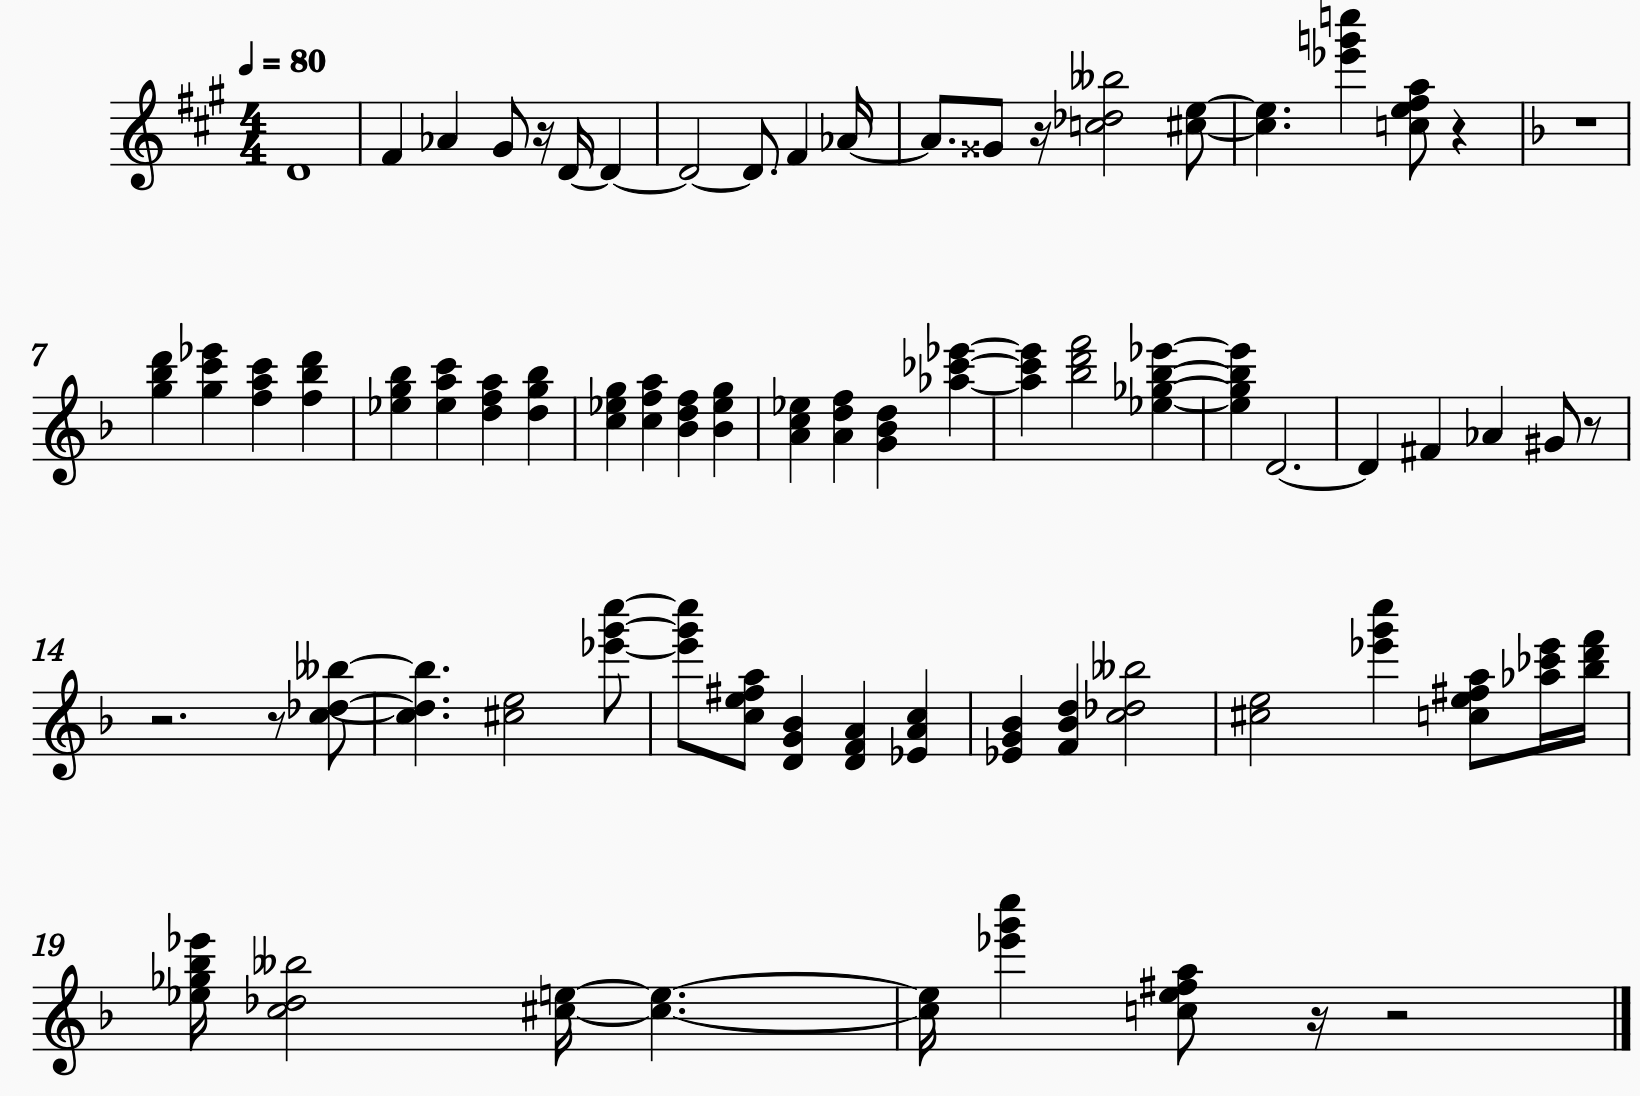
\includegraphics[width=\textwidth]{images/program1}
\caption{Example 1}
\label{fig:ex1}
\end{figure}

\newpage

\figref{fig:ex1} sounds rather atonal when played, but is presented to demonstrated the full complexity of MusAssist's features. Notice how MusAssist automatically breaks up the tied note rationally in mm. 19-20.

\figref{fig:ex2} sounds much more diatonic and pleasing to the ear, but is not as complex as \figref{fig:ex1}. Notice how the key signature at the beginning of the score does not change twice, though the command appears consecutively in the code. Also notice how  we represented the same A major triad in m. 2 in two ways: as a custom collection of enharmonic notes, and then as a chord template.


\section{Compiler Structure}

The MusAssist compiler is written in Haskell. Its high-level structure is as follows: 

\begin{enumerate}
  \item MusAssist concrete syntax is parsed into abstract syntax, represented as 
  Haskell algebraic data types. Parser combinators were chosen for their flexibility
  and easy customization. Parsec, an industrial strength parser library, is used, and 
  Parsec’s helper module Token handles lexing. The parse preserves the abstraction 
  level of all templates.

  \item Templates are expanded until the abstraction level is fully lowered to notes and
  rests. The result is abstract syntax whose low-level abstraction
  matches that of the target language MusicXML. 

  \item The low-level abstract syntax resulting from the fully expanded templates is 
  translated to MusicXML.
\end{enumerate}

The resulting MusicXML file can then be opened in music notation software, such as MuseScore,
for viewing and further editing. 

\section{Template Expansion Logic}
MusAssist's most powerful feature is its ability to formalize musical theoretical templates 
to automate their expansion so the user can specify them at the elevated level of abstraction 
of the musical structures they describe. This section summarizes the logic underlying the expansions.

\subsection{Chords}
\subsection{Cadences}
\subsection{Harmonic Sequences}

\section{Future Work}
Ideally, in the future MusAssist would support more complex musical states and elements including
custom time signature and mid-composition time signature changes (similar to the behavior
currently implemented for key signatures), clef changes within a part, multiple-clef parts (e.g.
piano), multiple voicing within a part, custom parts (i.e. instruments), and multiple part compositions.
Custom and changeable time signature would allow for the users to experiment with metric modulation,
something that is currently impossible with the fixed common time setup. Clef changes within a
part, both manual and automatic when a note extends too many ledger lines beyond a clef, would
allow the score to be more aesthetically formatted and readable for the user. Support for two-clef piano
would allow the MusAssist compiler to successfully modify how it generates cadences and harmonic
sequences to include the essential baseline, in addition to the harmonization already implemented.
Multiple voicing would allow for the user to create more complex musical lines, particularly with
counterpoint. The latter two goals (custom parts and multiple parts) are somewhat outside MusAs-
sist’s goal as a music compositional aid, as this extends beyond the realm of music theory. However,
users may enjoy this increased flexibility when composing. Furthermore, in line with its goal of
offering the user complex musical templates, it would be ideal for MusAssist to provide support for
key modulation; e.g. generating a sequence of chords that successfully modulates from one key to
another key. More complex/non-classical chords, such as all flavors of suspended, ninth, eleventh,
and thirteen chords (often seen in jazz) are a future goal as well. It would also be ideal for MusAssist
to be able to generate scales in any key, of any type (i.e. major, harmonic minor, octatonic etc),
and of any length. Finally, MusAssist would in the future support more complex rhythms where
any number of notes could be grouped over any number of beats (i.e. triplet, which is three eighths
over a quarter note, or a 4:3 rhythm of four eighths over three quarter notes)

\section{Conclusion}


% this inserts a column-break
%\pagebreak

\subsection{Title and Authors}
The title is 16~pt Times, bold, upper case, centered. Authors' names are centered. The lead author's name is to be listed first (left-most), and the co-authors' names after. If the addresses for all authors are the same, include the address only once, centered. If the authors have different addresses, put the addresses, evenly spaced, under each authors' name.

\subsection{First Page Copyright Notice}
Please include the copyright notice exactly as it appears here in the lower left-hand corner of the page. It is set in 8~pt Times, one column in width, and should not descend into the  page margins (i.e. it should keep clear of the 1" margin at the bottom of the page).

\subsection{Page Numbering, Headers and Footers}
Do not include headers, footers or page numbers in your submission. These will be added when the publications are assembled.

\section{Headings}
First level headings are in Times 12pt bold, centered with 1 line of space above the section head, and 1/2 space below it.  For a section header immediately followed by a subsection header, the space should be merged.

\subsection{Second Level Headings}
Second level headings are in Times 10~pt bold, flush left,
with 1 line of space above the section head, and 1/2 space below it.
The first letter of each significant word is capitalized.

\subsubsection{Third and further Level Headings}
Third level headings are in Times 10~pt italic, flush left, with 1/2 line of space above the section head, and 1/2 space below it. The first letter of each significant word is capitalized.

Using more than three levels of headings is strongly discouraged.

\pagebreak

\section{Equations, Figures, Footnotes}

\subsection{Equations}
Equations should be placed on separated lines and numbered.
The number should be on the right side, in parentheses.
\begin{equation}
E=mc^{2}.
\label{eq:Emc2}
\end{equation}

\subsection{Figures, Tables and Captions}
All artwork must be centered, neat, clean, and legible. All lines should be very dark for purposes of reproduction and artwork should not be hand-drawn. The proceedings will be distributed in electronic form only, therefore color figures are allowed. However, you may want to check that your figures are understandable even if they are printed in black-and-white.
\begin{table}[h]
 \begin{center}
 \begin{tabular}{|l|l|}
  \hline
  String Value & Numeric value \\
  \hline
  Hello ICMC & 2021 \\
  \hline
 \end{tabular}
\end{center}
 \caption{Table captions should be placed below the table.}
 \label{tab:example}
\end{table}

Numbers and captions of figures and tables always appear below the figure/table. Leave 1 line space between the figure or table and the caption. Figure and tables are numbered consecutively. Captions should be Times 10~pt. Place tables/figures in text as close to the reference as possible, and preferably at the top of the page.

\begin{figure}[h]
\centering
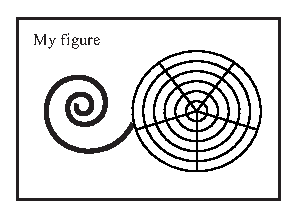
\includegraphics[width=0.9\columnwidth]{figure.eps}
\caption{Figure captions are placed below the figure, exactly like this.\label{fig:example}}
\end{figure}

Always refer to tables and figures in the main text, for example:
see Figure \ref{fig:example} and \tabref{tab:example}. 
Place Tables/Figures in text as close to the reference as possible.
Figures and tables may extend across both columns to a maximum width of 17.2cm.

Vectorial figures are preferred. 
When using {\texttt{Matlab}}, 
export using either Postscript or PDF format. 
Also, in order to optimize readability, the font size of text within a figure should be at list identical to footnote font size. If bitmap figures are used, please make sure that the resolution is enough for print quality. 

\subsection{Footnotes}
Indicate footnotes with a number in the text.\footnote{This is a footnote.}
Use 8~pt type for footnotes. Place the footnotes at the bottom of the page 
on which they appear. 
Precede the footnote with a 0.5~pt horizontal rule.

%\newpage

\section{Citations}
All bibliographical references should be listed at the end, inside a section named ``REFERENCES''.

References must be numbered {\ul {in order of appearance}}, {\em not} alphabetically. Please avoid listing references that do not appear in the text.

Reference numbers in the text should appear within square brackets, such as 
in~\cite{Someone:09} or~\cite{Someone:04,Someone:13}.

The reference format is the standard IEEE one. We recommend using BibTeX to create the reference list.


\section{Conclusions}
Please, submit full-length papers. Submission is fully electronic and automated through the Conference Management System. 
{\ul{Do not}} send papers directly by e-mail.

\begin{acknowledgments}
At the end of the Conclusions, acknowledgements to people, projects, funding agencies, etc. can be included after the second-level heading ``Acknowledgments'' (with no numbering).
\end{acknowledgments} 

%%%%%%%%%%%%%%%%%%%%%%%%%%%%%%%%%%%%%%%%%%%%%%%%%%%%%%%%%%%%%%%%%%%%%%%%%%%%%
%bibliography here
\bibliography{icmc2021template}

\end{document}
